% ===================================================================
%  Week 13 — Convolutional Neural Networks
% ===================================================================
\documentclass[10pt,aspectratio=169]{beamer}
% ===================================================================
%  Shared Beamer preamble for "Practical Image Processing"
%  English slides. Compile with pdfLaTeX.
% ===================================================================

\usetheme{metropolis}
\usepackage[T1]{fontenc}
\usepackage[utf8]{inputenc}
\usepackage{lmodern}
\usepackage{listings}
\usepackage{tcolorbox}
\usepackage{fontawesome5}
\usepackage{booktabs}
\usepackage{amsmath,amssymb}
\usepackage{tikz}
\usepackage{pgfplots}
\pgfplotsset{compat=1.17}
\usetikzlibrary{arrows.meta,positioning,shapes.geometric,fit,backgrounds,matrix}
\tcbuselibrary{skins,breakable}

% ---- Palette --------------------------------------------------------
\definecolor{coursePrimary}{HTML}{1B4965}   % deep blue
\definecolor{courseAccent}{HTML}{E76F51}    % coral
\definecolor{courseGood}{HTML}{2A9D8F}      % teal
\definecolor{courseBad}{HTML}{C0392B}       % red
\definecolor{courseInfo}{HTML}{2980B9}      % blue
\definecolor{codeBg}{HTML}{F5F6FA}
\definecolor{codeKw}{HTML}{8E44AD}
\definecolor{codeStr}{HTML}{2A9D8F}
\definecolor{codeCom}{HTML}{7F8C8D}

\setbeamercolor{frametitle}{bg=coursePrimary}
\setbeamercolor{progress bar}{fg=courseAccent}
\setbeamercolor{alerted text}{fg=courseAccent}
\metroset{block=fill,sectionpage=progressbar,numbering=fraction}

% ---- Code listings (Python is built into listings) -----------------
\lstdefinestyle{course}{
  backgroundcolor=\color{codeBg},
  basicstyle=\ttfamily\scriptsize,
  keywordstyle=\color{codeKw}\bfseries,
  stringstyle=\color{codeStr},
  commentstyle=\color{codeCom}\itshape,
  numberstyle=\tiny\color{codeCom},
  numbers=left, numbersep=6pt,
  showstringspaces=false, breaklines=true, breakatwhitespace=true,
  tabsize=4, columns=fullflexible,
  frame=single, framesep=4pt, rulecolor=\color{gray!30},
  keepspaces=true, upquote=true, language=Python,
}
\lstset{style=course}
\lstdefinelanguage{bash}{
  keywords={cd,pip,python,venv,source,import}, sensitive=true,
  morecomment=[l]{\#}, morestring=[b]', morestring=[b]",
}

% ---- Reusable callout boxes ----------------------------------------
\newtcolorbox{goodbox}[1][Good practice]{colback=courseGood!8,colframe=courseGood,
  fonttitle=\bfseries,title={\faCheck~#1},boxrule=0.6pt,left=4pt,right=4pt,top=3pt,bottom=3pt}
\newtcolorbox{badbox}[1][Pitfall]{colback=courseBad!8,colframe=courseBad,
  fonttitle=\bfseries,title={\faTimes~#1},boxrule=0.6pt,left=4pt,right=4pt,top=3pt,bottom=3pt}
\newtcolorbox{infobox}[1][Note]{colback=courseInfo!8,colframe=courseInfo,
  fonttitle=\bfseries,title={\faInfoCircle~#1},boxrule=0.6pt,left=4pt,right=4pt,top=3pt,bottom=3pt}
\newtcolorbox{mathbox}[1][Math]{colback=coursePrimary!6,colframe=coursePrimary,
  fonttitle=\bfseries,title={\faCalculator~#1},boxrule=0.6pt,left=4pt,right=4pt,top=3pt,bottom=3pt}

\newcommand{\keyidea}[1]{\begin{alertblock}{Key idea}#1\end{alertblock}}
\newcommand{\term}[1]{\textbf{\color{coursePrimary}#1}}
\newcommand{\code}[1]{\lstinline[basicstyle=\ttfamily\small]|#1|}

% ---- A helper to draw a small pixel grid, cells shaded by value ----
% \pixelgrid{ {10,20,120,200,240}, {30,60,130,180,230}, ... }
\newcommand{\pixelgrid}[1]{%
  \begin{tikzpicture}[font=\scriptsize,scale=0.6]
    \foreach \row [count=\ry] in {#1} {
      \foreach \val [count=\cx] in \row {
        \draw[gray,fill=coursePrimary!8] (\cx,-\ry) rectangle ++(1,-1);
        \node at (\cx+0.5,-\ry-0.5) {\val};
      }
    }
  \end{tikzpicture}}


\title{Convolutional Neural Networks}
\subtitle{Week 13 — Learning the filters instead of designing them}
\author{Practical Image Processing}
\date{Lecture 13 \textbullet\ 60--70 min}

\begin{document}

\maketitle

\begin{frame}{The big idea}
  \begin{columns}[T]
    \begin{column}{0.58\textwidth}
      \begin{itemize}
        \item Week 3: \emph{we} designed kernels (blur, Sobel) by hand.
        \item Week 12: hand-designed features (HOG) hit a ceiling.
        \item \alert{Today:} let the network \term{learn the kernels} from data — and learn the classifier at the same time.
      \end{itemize}
    \end{column}
    \begin{column}{0.42\textwidth}
      \begin{alertblock}{Today's real result}
        A small CNN reads digits (0--9) at \textbf{97\%} — the DocScan digit reader, trained from scratch.
      \end{alertblock}
    \end{column}
  \end{columns}
\end{frame}

\begin{frame}{Roadmap}\tableofcontents\end{frame}

% ==================================================================
\section{From kernels to learned filters}
% ==================================================================

\begin{frame}{Convolution: you already know it}
  \begin{itemize}
    \item Week 3: slide a small kernel over the image, multiply-and-sum $\rightarrow$ a filtered image.
    \item A Sobel kernel detects edges; a blur kernel smooths. \emph{We} chose the numbers.
    \item A \term{convolutional layer} is the same operation — but the kernel numbers are \term{learned}.
  \end{itemize}
  \keyidea{A CNN is ``convolution with kernels chosen by training instead of by hand.''}
\end{frame}

\begin{frame}{What the network learns}
  \begin{center}
  
\includegraphics[width=0.75\linewidth]{../assets/learned_filters.png}
  \end{center}
  \begin{itemize}
    \item These are the 8 first-layer $3\times3$ filters our CNN \emph{learned} for digits.
    \item Nobody designed them — gradient descent found edge/stroke detectors that help read digits.
    \item Early layers learn edges; deeper layers combine them into parts, then whole shapes.
  \end{itemize}
\end{frame}

\begin{frame}{Feature maps}
  \begin{itemize}
    \item Applying one learned filter to the image gives a \term{feature map}: where that pattern appears.
    \item A layer has many filters $\rightarrow$ many feature maps (a ``stack'' of pattern detectors).
    \item The next layer convolves over that stack, combining simple patterns into complex ones.
  \end{itemize}
  \begin{mathbox}
    Conv layer: input stack $\rightarrow$ (learned filters) $\rightarrow$ output stack of feature maps.
  \end{mathbox}
\end{frame}

% ==================================================================
\section{Anatomy of a CNN}
% ==================================================================

\begin{frame}{The building blocks}
  \begin{center}
  \begin{tabular}{@{}lll@{}}
    \toprule
    \textbf{Layer} & \textbf{Does} & \textbf{Why} \\
    \midrule
    Convolution & learned filters $\rightarrow$ feature maps & detect patterns \\
    ReLU & $\max(0,x)$, elementwise & add non-linearity \\
    Pooling & downsample (e.g. $2\times2$ max) & shrink, add invariance \\
    Fully-connected & flatten $\rightarrow$ class scores & make the decision \\
    Softmax & scores $\rightarrow$ probabilities & pick the class \\
    \bottomrule
  \end{tabular}
  \end{center}
  \keyidea{Conv+ReLU+Pool blocks stack up, ending in a classifier — the standard CNN recipe.}
\end{frame}

\begin{frame}{Why ReLU (non-linearity)?}
  \begin{itemize}
    \item Stacking pure convolutions is still just one big linear filter — no extra power.
    \item \term{ReLU} ($\max(0,x)$) inserts a non-linearity between layers.
    \item That lets deep stacks represent complex, curved decision boundaries.
  \end{itemize}
  \begin{mathbox}
    Without a non-linearity, ten conv layers collapse into one. ReLU is what makes ``deep'' meaningful.
  \end{mathbox}
\end{frame}

\begin{frame}{Why pooling?}
  \begin{itemize}
    \item \term{Max-pooling} keeps the strongest response in each small window, halving the size.
    \item Gives \term{translation tolerance}: a digit shifted a pixel still activates the same units.
    \item Shrinks computation and grows the \term{receptive field} of later layers.
  \end{itemize}
  \begin{goodbox}
    Pooling = ``I saw this pattern somewhere in this region,'' not ``exactly at this pixel.''
  \end{goodbox}
\end{frame}

\begin{frame}{Our digit CNN, end to end}
  \begin{itemize}
    \item Input $8\times8$ digit $\rightarrow$ Conv(8 filters)+ReLU+Pool $\rightarrow$ $4\times4$.
    \item $\rightarrow$ Conv(16 filters)+ReLU+Pool $\rightarrow$ $2\times2$ $\rightarrow$ flatten (64) $\rightarrow$ FC $\rightarrow$ 10 scores.
    \item Softmax turns the 10 scores into probabilities; the largest is the predicted digit.
  \end{itemize}
  \keyidea{Two conv blocks and one linear layer — tiny by modern standards, yet it reads digits at 97\%.}
\end{frame}

% ==================================================================
\section{Training a CNN}
% ==================================================================

\begin{frame}{How does it learn the filters?}
  \begin{enumerate}
    \item \term{Forward pass}: run an image through; get predicted probabilities.
    \item \term{Loss}: measure how wrong (\term{cross-entropy} between prediction and true label).
    \item \term{Backprop}: compute how each weight affected the loss (the gradient).
    \item \term{Update}: nudge every weight to reduce the loss (\term{gradient descent}).
  \end{enumerate}
  \keyidea{Repeat over many images and epochs; the filters gradually become good detectors.}
\end{frame}

\begin{frame}{Cross-entropy loss, intuitively}
  \begin{itemize}
    \item The network outputs a probability for each class. Cross-entropy is low when it puts high
          probability on the \emph{correct} class.
    \item Confidently wrong $\rightarrow$ huge loss. Correct and confident $\rightarrow$ near-zero loss.
    \item Training minimizes the average loss over the data.
  \end{itemize}
  \begin{mathbox}
    Loss for one sample $= -\log(p_{\text{true class}})$. Push $p_{\text{true}}\to 1$.
  \end{mathbox}
\end{frame}

\begin{frame}{Training in action}
  \begin{columns}[T]
    \begin{column}{0.55\textwidth}\begin{center}
      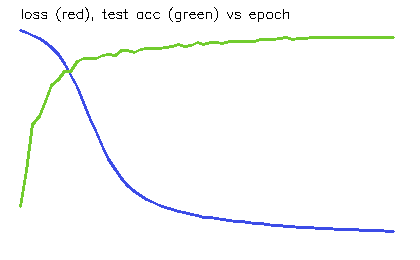
\includegraphics[width=0.98\linewidth]{../assets/training_curve.png}
    \end{center}\end{column}
    \begin{column}{0.45\textwidth}
      \begin{itemize}
        \item Red: training loss falls each epoch.
        \item Green: test accuracy climbs, then plateaus near 0.97.
        \item Watching both curves is how you spot under/over-fitting live.
      \end{itemize}
    \end{column}
  \end{columns}
\end{frame}

\begin{frame}{Mini-batches, epochs, learning rate}
  \begin{itemize}
    \item \term{Mini-batch}: update on a small group of images at a time (we used 128) — faster, smoother.
    \item \term{Epoch}: one full pass over the training set. We ran 60.
    \item \term{Learning rate}: step size of each update. Too big $\rightarrow$ diverges; too small $\rightarrow$ crawls.
  \end{itemize}
  \begin{badbox}
    Most training failures are a bad learning rate. If loss explodes or won't move, change it first.
  \end{badbox}
\end{frame}

% ==================================================================
\section{Results}
% ==================================================================

\begin{frame}{Reading digits — the DocScan payoff}
  \begin{center}
  
\includegraphics[width=0.85\linewidth]{../assets/predictions.png}
  \end{center}
  \vspace{2pt}
  Test digits with the CNN's prediction (green = correct). This is the meter-digit reader DocScan needs.
\end{frame}

\begin{frame}{CNN vs classical — an honest comparison}
  \begin{center}
  \begin{tabular}{@{}lc@{}}
    \toprule
    \textbf{Method} & \textbf{Test accuracy (digits)} \\
    \midrule
    CNN (learned filters) & 0.97 \\
    SVM on raw pixels & 0.99 \\
    \bottomrule
  \end{tabular}
  \end{center}
  \begin{itemize}
    \item On \emph{easy}, clean $8\times8$ digits, classical ML is already excellent — CNN isn't magic here.
    \item The CNN's real advantage shows on \emph{hard, large, varied} images — and with \term{transfer learning} (Week 14).
  \end{itemize}
\end{frame}

\begin{frame}{When do CNNs really win?}
  \begin{itemize}
    \item Large, varied datasets where hand features can't capture the variation.
    \item Problems where the useful features are unknown (the network discovers them).
    \item Recall Week 12: HOG+SVM plateaued at 48\% on look-alike cars — that's where learned features help.
  \end{itemize}
  \keyidea{Small clean problem $\rightarrow$ classical is fine. Big messy problem $\rightarrow$ deep learning pulls ahead.}
\end{frame}

% ==================================================================
\section{In-class exercise}
% ==================================================================

\begin{frame}{\faPen~In-class exercise (10 min)}
  \begin{infobox}[Reason about the architecture]
  \end{infobox}
  \begin{enumerate}
    \item How is a convolutional layer related to the Sobel kernel from Week 3?
    \item Why won't stacking convolutions \emph{without} ReLU give a more powerful model?
    \item Our CNN got 0.97 and the SVM 0.99 on digits. Does that mean CNNs are worse? Explain.
  \end{enumerate}
\end{frame}

\begin{frame}{\faPen~Debrief}
  \begin{itemize}
    \item (1) Both convolve a small kernel over the image; Sobel's numbers are fixed, the CNN's are \term{learned}.
    \item (2) Composing linear operations is still linear — \term{ReLU}'s non-linearity is what adds power.
    \item (3) No — on easy clean data classical ML is already near-perfect; CNNs win on hard, varied,
          large-scale data and via transfer learning.
  \end{itemize}
  \keyidea{Match the tool to the problem. The CNN's power is learned features — it pays off when the problem is hard.}
\end{frame}

% ==================================================================
\section{Deep dive}
% ==================================================================

\begin{frame}{The feature hierarchy}
  \begin{itemize}
    \item Layer 1: edges and simple strokes (like the learned filters we saw).
    \item Layer 2--3: corners, curves, digit parts (loops, junctions).
    \item Deeper: whole-shape detectors that fire for a specific digit.
  \end{itemize}
  \keyidea{A CNN builds complexity gradually — simple parts combine into meaningful wholes, all learned.}
\end{frame}

\begin{frame}{Regularization: keeping CNNs honest}
  \begin{itemize}
    \item CNNs have many parameters $\rightarrow$ they can overfit (Week 12's lesson returns).
    \item \term{Dropout}: randomly zero some activations during training so the net can't rely on any one.
    \item \term{Data augmentation}: random shifts/rotations of training images — free extra data, more invariance.
    \item \term{Weight decay}: penalize large weights to keep the model simple.
  \end{itemize}
\end{frame}

\begin{frame}{Why CNNs need a GPU (and lots of data)}
  \begin{itemize}
    \item Millions of multiply-adds per image; a GPU does them massively in parallel.
    \item Deep nets have millions of parameters — they need many examples to fit without overfitting.
    \item Our digit net is tiny and trains in seconds; ImageNet-scale nets train for days.
  \end{itemize}
  \begin{goodbox}
    Small data + deep net = overfitting. Next week's \term{transfer learning} fixes exactly this.
  \end{goodbox}
\end{frame}

\begin{frame}[fragile]{A CNN in PyTorch}
\begin{lstlisting}[language=Python]
class DigitCNN(nn.Module):
    def __init__(self):
        super().__init__()
        self.c1 = nn.Conv2d(1, 8, 3, padding=1)
        self.c2 = nn.Conv2d(8, 16, 3, padding=1)
        self.pool = nn.MaxPool2d(2)
        self.fc = nn.Linear(16*2*2, 10)
    def forward(self, x):
        x = self.pool(torch.relu(self.c1(x)))
        x = self.pool(torch.relu(self.c2(x)))
        return self.fc(x.flatten(1))
\end{lstlisting}
  Conv $\rightarrow$ ReLU $\rightarrow$ Pool, twice, then a linear classifier. That is the whole digit reader.
\end{frame}

% ==================================================================
\section{Wrap-up}
% ==================================================================

\begin{frame}{What you should now be able to do}
  \begin{itemize}
    \item Explain a CNN as convolution with \emph{learned} filters, plus ReLU, pooling, and a classifier.
    \item Describe how training works: forward, loss, backprop, gradient descent.
    \item Read training curves and recognize the role of batches, epochs, learning rate.
    \item Judge honestly when a CNN beats classical ML — and when it doesn't.
  \end{itemize}
\end{frame}

\begin{frame}{This week's deliverable}
  \begin{alertblock}{Due before Week 14 (see \code{project/})}
    \begin{enumerate}
      \item Train the small digit CNN; report test accuracy and show the training curve.
      \item Visualize the learned first-layer filters; describe what they detect.
      \item Compare to a classical baseline (SVM/k-NN) on the same digits.
      \item Reflect: on your data, when would you expect a CNN to beat classical features?
    \end{enumerate}
  \end{alertblock}
\end{frame}

\begin{frame}[standout]
  A CNN learns the filters Week 3 made us design.\\[4pt]
  \normalsize Convolution + ReLU + pooling, trained end to end — features and classifier together.
\end{frame}

\end{document}
